\documentclass[11pt]{scrartcl}
\usepackage{graphicx}
\usepackage{tikz}
\usetikzlibrary{angles,quotes}
\usetikzlibrary{patterns}
\usetikzlibrary{calc}
\usepackage{tkz-euclide}
\graphicspath{{./}}
\usepackage[sexy]{evan}
\usepackage[normalem]{ulem}
\usepackage{hyperref}
\usepackage{mathtools}
\hypersetup{
    colorlinks=true,
    linkcolor=blue,
    filecolor=magenta,      
    urlcolor=cyan,
    pdftitle={Educational PDF by Azzam},
    pdfpagemode=FullScreen,
    }

\usepackage{listings}
\usepackage{xcolor}
\lstset { %
    language=C++,
    backgroundcolor=\color{black!5}, % set backgroundcolor
    %basicstyle=\footnotesize,% basic font setting
}
 
\renewcommand{\baselinestretch}{1.5}

\addtolength{\oddsidemargin}{-0.4in}
\addtolength{\evensidemargin}{-0.4in}
\addtolength{\textwidth}{0.8in}
% \addtolength{\topmargin}{-0.2in}
% \addtolength{\textheight}{1in} 

\setlength{\parindent}{0pt}

\usepackage{pgfplots}
\pgfplotsset{compat=1.15}
\usepackage{mathrsfs}
\usetikzlibrary{arrows}

\begin{document}
\title{Basic Lessons on High School Olympiad 1} % Beginner
\date{\today}
\author{Azzam L. H.}
\maketitle
\renewcommand*\contentsname{Daftar Isi}
\tableofcontents

\newpage
\section{Aljabar}
\subsection{Pemfaktoran dan Penguraian}
Tips: Jangan dihafal secara sengaja, tetapi banyak-banyaklah latihan soal, nanti hafal sendiri :D.
	
	Untuk $x,y,z \in \CC$.

        \subsubsection{\textit{Basic} yang paling sering muncul}
        \begin{enumerate}
            \item $x^2-y^2 = (x+y)(x-y)$.
	    \item $(x+y)^2 = x^2+2xy+y^2$.
	    \item $(x-y)^2 = x^2-2xy+y^2$.
            \item $(x+y)^3 = x^3+y^3+3xy(x+y) = x^3+3x^2y+3xy^2+y^3$. 
	    \item $(x-y)^3 = x^3-y^3+3xy(x-y) = x^3-3x^2y+3xy^2-y^3$. 
	    \item $x^3-y^3 = (x-y)(x^2+xy+y^2)$.
	    \item $x^3+y^3 = (x+y)(x^2-xy+y^2)$.
	    \item $x^n-y^n = (x-y)(x^{n-1}+x^{n-2}y+x^{n-3}y^2+\dots+xy^{n-2}+y^{n-1})$ untuk $n \in \NN$.
	    \item $x^n+y^n = (x+y)(x^{n-1}-x^{n-2}y+x^{n-3}y^2-\dots+xy^{n-2}+y^{n-1})$ untuk $n$ bilangan asli \textbf{ganjil}.
        \end{enumerate}

        \subsubsection{Lebih \textit{Advanced}}
	\begin{enumerate}
	    \item $(x+y+z)^2 = x^2+y^2+z^2+2xy+2yz+2zx$.
	    \item $x^2+y^2+z^2+xy+yz+zx = \frac12(x+y)^2+\frac12(y+z)^2+\frac12(z+x)^2$.
	    \item $x^2+y^2+z^2-xy-yz-zx = \frac12(x-y)^2+\frac12(y-z)^2+\frac12(z-x)^2$.
	    \item $x^3+y^3+z^3-3xyz = (x+y+z)(x^2+y^2+z^2-xy-yz-zx)$.
	    \item $(x+1)(y+1)(z+1)=xyz+xy+yz+zx+x+y+z+1$.
	    \item (Identitas Sophie Germain) $x^4+4y^4=(x^2+2xy+2y^2)(x^2-2xy+2y^2)$.
	    \item (Ekspansi Binomial) $(x+y)^n = {n \choose 0}x^ny^0 + {n \choose 1}x^{n-1}y^1+{n \choose 2}x^{n-2}y^2 + \dots + {n \choose n}x^0y^n$.
	    \item (Fermat Two Square Identity / Brahmagupta-Fibonacci Identity)\\
        $(a^2+b^2)(c^2+d^2)=(bc+ad)^2+(bd-ac)^2$ untuk $a,b,c,d \in \RR$.
	\end{enumerate}

 \subsection{Latihan Soal Pemfaktoran dan Manipulasi Aljabar}
\begin{enumerate}
    \item  Nilai dari $\sqrt{5050^2-4950^2}$ adalah \dots

    \item (OSP 2008) Jika $0 < b < a$ dan $a^2+b^2=6ab$, maka nilai $\dfrac{a+b}{a-b}=\dots$
    
    \item Jika $x > 0$ dan $x + \dfrac{1}{x} =  5$, maka nilai $x^3+\dfrac{1}{x^3}$ adalah \dots
    
    \item (OSK 2017) Diketahui $x-y=10$ dan $xy=10$. Nilai $x^4+y^4$ adalah \dots
    
    \item (OSK 2018) Diketahui $x$ dan $y$ bilangan prima dengan $x < y$, dan $x^3+y^3+2018=30y^2-300y+3018$. Nilai $x$ yang memenuhi adalah \dots
    
    \item Jika $a+b+c=0$ untuk suatu bilangan riil $a,b,c$, buktikan bahwa $a^3+b^3+c^3=3abc$.
    
    \item Jika $x=2021^3-2019^3$, maka nilai $\sqrt{\dfrac{x-2}{6}}$ adalah \dots

    \item (AIME 1987)
    Tentukan nilai sederhana dari $\dfrac{(10^4+324)(22^4+324)(34^4+324)(46^4+324)(58^4+324)}{(4^4+324)(16^4+324)(28^4+324)(40^4+324)(52^4+324)}$

    \item (OSK 2017) Jika $\dfrac{(a-b)(c-d)}{(b-c)(d-a)}=-\dfrac{4}{7}$, maka nilai dari $\dfrac{(a-c)(b-d)}{(a-b)(c-d)}$ adalah \dots

    \item (OSK 2019) Diketahui $a+2b=1$, $b+2c=2$, dan $b \neq 0$. Jika $a+nb+2018c = 2019$ maka nilai $n$ adalah \dots

    \item (OSK 2019) Misalkan $a = 2\sqrt{2} - \sqrt{8-4\sqrt{2}}$ dan $b = 2\sqrt{2} + \sqrt{8-4\sqrt{2}}$. Jika $\dfrac{a}{b}+\dfrac{b}{a}=x+y\sqrt{2}$ dengan $x,y$ bulat, maka nilai $x+y$ adalah \dots

    \item (OSK 2015) Diketahui bilangan real positif $a$ dan $b$ memenuhi persamaan
    \begin{align*}
        a^4+a^2b^2+b^4=6 \text{ dan } a^2+ab+b^2=4
    \end{align*}
    Nilai dari $a + b$ adalah \ldots

    \item (OSK 2022) Diketahui $a,b,c,d$ bilangan real positif yang memenuhi $a>c$, $d>b$, dan 
    $$3a^2+3b^2=3c^2+3d^2=4ac+4bd.$$
    Nilai $\dfrac{12(ab+cd)}{ad+bc}=\dots$ 
\end{enumerate}

\subsection{Eksponen}
Untuk $a,b,c \in RR$
\begin{enumerate}
    \item $a^0=1$ untuk $a \neq 0$.
    \item $a^n =  \underbrace{a \cdot a \cdot \ldots \cdot a}_{n \text{ kali}}$ untuk $n \in \NN$.
    \item $a^b\cdot a^c=a^{b+c}$.
    \item $a^b\cdot c^b = (ac)^b$.
    \item $\dfrac{a^b}{a^c}=a^{b-c}$ untuk $a\neq 0$.
    \item $(a^b)^c=a^{bc}$.
    \item $a^{-b} = \dfrac{1}{a^b}$ untuk $a \neq 0$.
    \item $\sqrt[n]{a^b}=a^{\dfrac{b}{n}}$ untuk $n \in \ZZ_{\ge 2}$
\end{enumerate}
\subsection{Latihan Soal Eksponen}
\begin{enumerate}
    \item Carilah jumlah semua bilangan bulat positif $a$ yang memenuhi $a^{(a-1)^{(a-2)}}=a^{a^2-3a+2}$.
    
    \item Carilah jumlah seluruh solusi real $x$ yang memenuhi $(x^2+5x+5)^{x^2-10x+21}=1.$
    
    \item Jika $5^x=6^y=30^7$, berapakah nilai $\dfrac{xy}{x+y}$?
\end{enumerate}

\newpage
\section{Teori Bilangan}
Pada dasarnya aljabar tetapi di ranah bilangan bulat (atau rasional).
\subsection{Paritas Penjumlahan dan Perkalian antara Dua Bilangan}
Paritas dalam konteks ini adalaha "genap-ganjil" nya suatu bilangan.
    \begin{enumerate}
        \item Bilangan Ganjil $\pm$ Bilangan Ganjil = Bilangan Genap 
        \item Bilangan Genap $\pm$ Bilangan Ganjil = Bilangan Ganjil 
        \item Bilangan Genap $\pm$ Bilangan Genap = Bilangan Genap 
        \item Bilangan Ganjil $\times$ Bilangan Ganjil = Bilangan Ganjil 
        \item Bilangan Ganjil $\times$ Bilangan Genap = Bilangan Genap 
        \item Bilangan Genap $\times$ Bilangan Genap = Bilangan Genap
    \end{enumerate}
    Dari sifat-sifat perkalian dua bilangan akan didapat bahwa bilangan genap tidak mungkin membagi bilangan ganjil sedangkan bilangan ganjil mungkin membagi bilangan genap. 


    
\subsection{Keterbagian}
    Untuk bilangan bulat $a \neq 0$ serta bilangan bulat $b,c,x$ dan $y$, notasikan $a \mid b$ sebagai $a$ membagi $b$. Lalu, $a$ dan $b$ relatif prima atau $a$ dan $b$ koprima (coprime) jika dan hanya jika $FPB(a,b)=1$.
    \begin{enumerate}
        \item Kita dapat menyatakan semua bilangan bulat $c = pq+r$ untuk suatu bilangan bulat $q$ dimana $0 \le r < q$. Jadi, saat $c$ dibagi $p$, maka hasil baginya adalah $q$ dan sisa baginya adalah $r$.
        \item Terdapat suatu bilangan bulat $x$ dimana $a \mid b \iff b=ax$.
        \item $a \mid a$.
        \item $a \mid 0$.
        \item $1 \mid a$.
        \item $a \mid b \implies a \mid bc$.
        \item Untuk $a,b \neq 0$ maka $ab \mid c \implies a \mid c \text{ dan } b \mid c$.
        \item $a \mid b \text{ dan } b \mid c \implies a \mid c$.
        \item $a \mid b \text{ dan } a \mid c \implies a \mid bx + cy$.
        \item $a \mid b \text{ dan } a \mid c \implies a \mid b+c$.
        \item $a \mid b \text{ dan } a \mid c \implies a \mid b-c$.
        \item Untuk $x \neq 0$ maka $a \mid b \iff xa \mid xb$.
        \item $a \mid b$ dan $b \neq 0$ maka $|a| \le |b|$.
        \item $a \mid bc$ dan $FPB(a,b)=1$ maka $a\mid c$.
    \end{enumerate}


    
\subsection{Aritmatika Modular}
    Untuk suatu bilangan asli $m$ dan bilangan bulat $a,b,c$ dan $d$, notasikan $m\mid a-b \iff a \equiv b \mod m$ (dibaca $a$ kongruen $b$ modulo $m$). Simpelnya $a \equiv b \mod m$ adalah $a$ dibagi $m$ bersisa $b$. Contohnya $5 \equiv 2 \mod 3$. $13 \equiv 3 \mod 5$. $10 \equiv -2 \mod 12$.
    \begin{enumerate}
        \item $a \equiv a \mod m$.
        \item $a \equiv 0 \mod m \iff m\mid a$.
        \item $a \equiv b \mod m \iff b \equiv a \mod m$.
        \item $a \equiv b \mod m \text{ dan } b \equiv c \mod m \implies a \equiv c \mod m$.
        \item Jika $a \equiv b \mod m$ dan $d\mid m$ maka $a \equiv b \mod d$.
        \item Untuk semua bilangan asli $k$, $a \equiv b \mod m \iff a^k \equiv b^k \mod m$.
        \item $a \equiv b \mod m \text{ dan } c \equiv d \mod m \implies a+c \equiv b+d \mod m$.
        \item $a \equiv b \mod m \text{ dan } c \equiv d \mod m \implies a-c \equiv b-d \mod m$.
        \item $a \equiv b \mod m \text{ dan } c \equiv d \mod m \implies ac \equiv bd \mod m$.
        \item $\forall k\in \ZZ^+, (am+b)^k \equiv b^k \mod m$.
        \item Jika $ca \equiv cb \mod m$ dengan $FPB(c,m)=1$, maka $a \equiv b \mod m$.
    \end{enumerate}
    
    Catatan: Penggunaan sifat nomor 8 dapat dimodifikasi sehingga menjadi konsep \textbf{Chinese Remainder Theorem}.

\subsection{Latihan Soal Aritmatika Modular}
\begin{enumerate}    
    \item (AIME 1986) Tentukan bilangan asli $n$ terbesar sehingga $n+10 \mid n^3+100$.
    
    \item Tentukan digit satuan dari $7^{7^7}$.
    
    \item Jika $S=1!+2!+3!+\dots+2021!$, tentukan sisa $S$ saat dibagi 6.
    
    \item (OSK 2009) Sisa saat $10^{999999999}$ saat dibagi oleh 7 adalah \dots
    
    \item (OSK 2011) Bilangan asli terkecil $n>2011$ yang bersisa 1 jika dibagi $2,3,4,5,6,7,8,9,10$ adalah \dots.

    \item (OSK 2015) Bilangan $x$ adalah bilangan bulat positif terkecil yang membuat
    \[31^n + x \cdot 96^n\]
    merupakan kelipatan 2015 untuk setiap bilangan asli $n$. Nilai $x$ adalah \ldots
\end{enumerate}
\subsection{Uji habis dibagi}
    Trik yang suatu saat dapat membuat hidup anda bahagia :D. Semua rumus ini dapat dibuktikan dengan aritmatika modular.
    \begin{enumerate}
        \item Bilangan $x$ genap jika dan hanya jika digit terakhir $x$ genap.
        \item $3 \mid x$ jika dan hanya jika jumlah digit-digitnya habis dibagi $3$. Contohnya 2931 habis dibagi 3 karena $2+9+3+1=15$ habis dibagi 3.
        \item $9 \mid x$ jika dan hanya jika jumlah digit-digitnya habis dibagi $9$.
        \item $x$ habis dibagi 5 jika dan hanya jika digit terakhir $x$ adalah $0$ atau $5$.
        \item $x$ habis dibagi 11 jika dan hanya jika jumlah selang-seling (alternate sums) dari digit-digitnya habis dibagi 11. Contoh: 945351 habis dibagi 11 karena $9-4+5-3+5-1=11$ habis dibagi 11. 121 habis dibagi 11 karena $1-2+1=0$ habis dibagi 11.
    \end{enumerate}


    
        
\newpage    
\section{Kombinatorika}

Notasikan $n!=n \times (n-1) \times (n-2) \times \dots \times 3 \times 2 \times 1$ (dibaca $n$ faktorial) dengan $1!=0!=1$.

\subsection{Permutasi}
Permutasi $k$ unsur dari $n$ unsur adalah (urutan diperhatikan)
$$_nP_k = P_k^n = \dfrac{n!}{(n-k)!}.$$
\subsection{Kombinasi}
Kombinasi $k$ unsur dari $n$ unsur adalah (urutan tak diperhatikan)
$${n \choose k}=_nC_k = C_k^n = \dfrac{n!}{k!(n-k)!}.$$
\subsection{Latihan Soal Kombinasi}
\begin{enumerate}   
    \item  Carilah banyaknya menempatkan 3 benteng (rooks) pada papan catur $5 \times 5$ sehingga tidak ada dua catur yang dalam posisi dapat saling menyerang.

    \item Carilah banyaknya kuadrupel terurut bilangan ganjil positif $(x_1, x_2, x_3, x_4)$ yang memenuhi $x_1 + x_2 + x_3 + x_4 = 98$.

    \item Perhatikan gambar berikut. 
    
    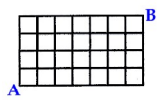
\includegraphics[width=0.2\linewidth]{Soal/Combinatorics/shortestPath.PNG} 
    
    Jika seseorang akan berjalan dari titik A ke titik B. Ada berapa banyak cara jalan terpendek yang dapat dipilihnya ?

    \item (OSK 2010) Banyaknya himpunan $X$ yang memenuhi 
    $$\{1,2,\dots,1000\} \subseteq X \subseteq \{1,2,\dots,2010\}.$$

    \item (OSP 2010) Bilangan asli enam digit $abcdef$ dengan $a > b > c \ge d > e > f$ ada sebanyak \dots
    
    \item (OSK 2017)
	Sebuah hotel mempunyai kamar bernomor 000 sampai dengan 999. Hotel tersebut menerapkan aturan aneh sebagai berikut: jika suatu kamar berisi tamu, dan sembarang dua digit nomor kamar tersebut dipertukarkan tempatnya, maka diperoleh nomor kamar yang sama atau nomor kamar yang tidak berisi tamu. Maksimal banyaknya kamar yang berisi tamu adalah \dots
\end{enumerate}
\subsection{Permutasi Siklis}
$n$ objek ditaruh mengelilingi lingkaran maka banyak cara menyusunnya adalah
$$P_{siklis} =\dfrac{n!}{n} = (n-1)!$$
\subsection{Stars and Bars}
Banyaknya solusi bulat non-negatif $(x_1,x_2,\dots,x_k)$ dari sistem persamaan $x_1+x_2+\dots+x_k=n$ adalah
$${n+k-1 \choose k-1}.$$
Banyaknya solusi bulat positif $(x_1,x_2,\dots,x_k)$ dari sistem persamaan $x_1+x_2+\dots+x_k=n$ adalah
$${n-1 \choose k-1}.$$

\subsection{Latihan Soal Stars and Bars}
\begin{enumerate}
    \item Carilah banyaknya kuadrupel terurut bilangan ganjil positif $(x_1, x_2, x_3, x_4)$ yang memenuhi $x_1 + x_2 + x_3 + x_4 = 98$.
\end{enumerate}

\newpage
\section{Geometri}
Pada dasarnya geometri di olimpiade matematika SMA "hanya" tentang lingkaran dan segitiga dua dimensi (Soal bangun tiga dimensi hampir ngga pernah dikeluarin untuk lomba tingkat SMA).
    
\subsection{Garis, Segmen Garis, Sinar (Bukan Vektor!)}
    Perlu ditekankan bahwa \textbf{garis tidak sama dengan ruas garis}. Garis panjangnya tak hingga, sedangkan ruas garis atau segmen garis panjangnya terbatas. Gambar di bawah terdiri dari \textbf{garis AB, segmen garis CD, sinar EF}.
\begin{center}
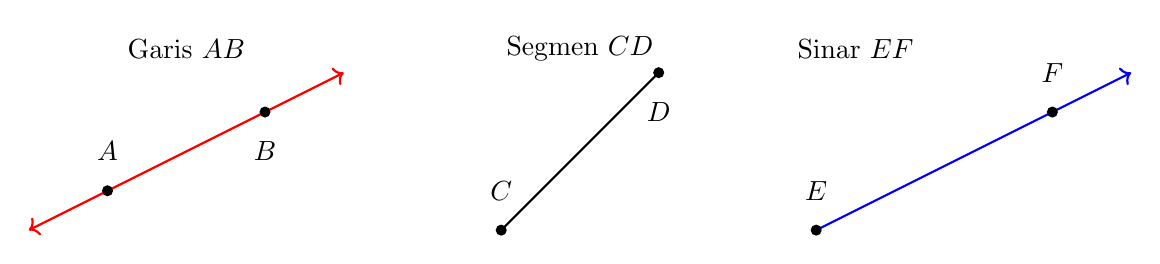
\begin{tikzpicture}
    % Draw a line
    \draw[red, thick, <->] (-4,-1) -- (0,1);
    \node at (-2,1.3) {Garis $AB$};
    \fill (-3,-0.5) circle (2pt);
    \fill (-1,0.5) circle (2pt);
    \node at (-3,-0) {$A$};
    \node at (-1,0) {$B$};

    % Draw a segment
    \draw[thick] (2,-1) -- (4,1);
    \node at (3,1.3) {Segmen $CD$};
    \fill (2,-1) circle (2pt);
    \fill (4,1) circle (2pt);
    \node at (2,-0.5) {$C$};
    \node at (4,0.5) {$D$};

    % Draw a ray
    \draw[blue, thick, ->] (6,-1) -- (10,1);
    \node at (6.5,1.3) {Sinar $EF$};
    \fill (6,-1) circle (2pt);
    \fill (9,0.5) circle (2pt);
    \node at (6,-0.5) {$E$};
    \node at (9,1) {$F$};
\end{tikzpicture}
\end{center}
\subsection{Lingkaran}

\begin{center}
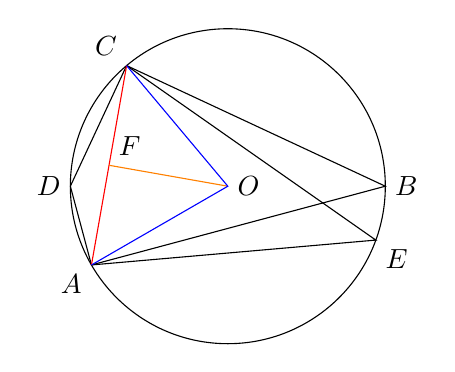
\begin{tikzpicture}
\coordinate (O) at (0,0);
\coordinate (B) at (0:2cm);
\coordinate (A) at (210:2cm);
\coordinate (D) at (180:2cm);
\coordinate (C) at (130:2cm);
\coordinate (E) at (-20:2cm);

\draw (O) circle (2cm);

\draw (A) -- (B) -- (C) -- (D) -- cycle;
\draw (A) -- (E) -- (C);
\draw[red] (A) -- (C);

\tkzDefPointBy[projection=onto A--C](O) \tkzGetPoint{F}
\draw[orange] (O) -- (F);
\draw[blue] (C) -- (O) -- (A);

\node[right] at (B) {$B$};
\node[below left] at (A) {$A$};
\node[left] at (D) {$D$};
\node[above left] at (C) {$C$};
\node[below right] at (E) {$E$};
\node[right] at (O) {$O$};
\node[above right] at (F) {$F$};
\end{tikzpicture}
\end{center}

    
Misalkan $O$ pusat lingkaran $\Gamma$ dan $A,B,C,D,E$ adalah sembarang titik pada lingkaran $\Gamma$ seperti pada gambar.
\begin{enumerate}
    \item $CO=OA$ adalah jari-jari dengan $\angle ACO = \angle OAC$.
    \item Misalkan titik $F$ adalah titik tengah tali busur $CA$, maka $OF \perp CA$ atau $OF$ tegak lurus dengan $CA$, dengan kata lain, $F$ adalah proyeksi titik $O$ ke $CA$
    \item (Sudut keliling-sudut pusat) Untuk$\angle COA = 2\angle CBA$.
    \item (sudut keliling) $\angle CBA = \angle CEA$.
    \item $ABCD$ adalah segiempat tali busur atau segiempat siklis  atau $A,B,C,D$ terletak di lingkaran (seperti pada gambar) jika dan hanya jika $\angle CBA + \angle ADC = 180^\circ$ atau $\angle ABD = \angle ACD$.
\end{enumerate}
\subsection{Segitiga}
Pada segitiga $ABC$ seperti gambar berikut:
\begin{center}
\begin{tikzpicture}
    % Define the coordinates of the vertices
    \coordinate (A) at (0,0);
    \coordinate (B) at (8,0);
    \coordinate (C) at (1.5,4);
    
    % Draw the triangle
    \draw (A) -- (B) -- (C) -- cycle;
    
    % circumcircle
    \tkzCircumCenter(A,B,C)\tkzGetPoint{O}
    \tkzDrawPoint(O)
    \tkzDrawCircle(O,A)
    
    % incircle
    \tkzDefCircle[in](A,B,C)\tkzGetPoint{I}\tkzGetLength{rIN}
    \tkzDrawPoint(I)
    \tkzDrawCircle[R](I,\rIN pt)
    
    % angle bisector
    \tkzDrawBisector[blue](B,A,C)\tkzGetPoint{E}
    \tkzDrawCircle[R](E,1 pt)
    
    %altitude
    \tkzDefPointBy[projection=onto B--C](A) \tkzGetPoint{D}
    \tkzDefPointBy[projection=onto B--A](C) \tkzGetPoint{C1}
    \tkzInterLL(A,D)(C,C1) \tkzGetPoint{H}
    \tkzDrawPoints(H) \tkzLabelPoints[below right](H)
    \tkzDrawSegment[red](A,D)
    \tkzDrawSegment[red](C,C1)

    %garis sumbu
    \tkzDefPointBy[projection=onto B--C](O) \tkzGetPoint{M}
    \tkzDefPointBy[homothety=center O ratio 3.2](M) \tkzGetPoint{M1}
    \tkzDefPointBy[homothety=center O ratio -3.2](M) \tkzGetPoint{M2}
    \tkzDrawSegment(M1,M2)
    \tkzDefPointBy[projection=onto B--A](O) \tkzGetPoint{M3}

    %centroid
    \tkzDrawSegment[green](A,M)
    \tkzDrawSegment[green](C,M3)
    \tkzInterLL(A,M)(C,M3) \tkzGetPoint{G}
    \tkzDrawPoints(G) \tkzLabelPoints[below right](G)
    
    % Label the vertices
    \node[below left] at (A) {$A$};
    \node[below right] at (B) {$B$};
    \node[above] at (C) {$C$};
    \node[below right] at (I) {$I$};
    \node[right] at (O) {$O$};
    \node[above right] at (E) {$E$};
    \node[above] at (D) {$D$};
    \node[right] at (M) {$M$};
\end{tikzpicture}
\end{center}
\begin{enumerate}
    \item Garis bagi $AE$ yaitu garis yang membagi dua sudut $A$ sama besar sehingga $\angle BAE = \angle EAC$. 
    \item Garis berat $AM$ dengan $M$ adalah titik tengah $BC$.
    \item Garis tinggi $AD$ adalah garis yang tegak lurus dengan $BC$. $D$ biasa disebut dengan proyeksi $A$ ke $BC$.
    \item Garis $OM$ adalah salah satu garis sumbu segitiga $ABC$, yaitu garis yang melewati titik tengah sisi segitiga dan tegak lurus dengan sisi itu.
    \item Pertemuan atau perpotongan ketiga garis tinggi segitiga $ABC$ adalah titik tinggi, dalam gambar ini adalah $H$ (orthocenter).
    \item Pertemuan atau perpotongan ketiga garis bagi segitiga $ABC$ adalah titik bagi atau titik pusat lingkaran dalam (incircle) segitiga $ABC$ dalam gambar ini adalah $I$ (incenter).
    \item Pertemuan atau perpotongan ketiga garis berat segitiga $ABC$ adalah titik berat (centroid).
    \item Pertemuan atau perpotongan ketiga garis sumbu segitiga $ABC$ adalah titik pusat lingkaran luar (circumcircle) segitiga $ABC$ yang dalam gambar ini adalah $O$ (circumcenter).
    \item Berlaku \textbf{ketaksamaan segitiga} yaitu $AB+BC>CA$, $BC+CA>AB$, dan $CA+AB>BC$. Selain itu juga berlaku $|AB-BC|<CA$, $|BC-CA|<AB$, dan $|CA-AB|<BC$.
\end{enumerate}
\subsection{Kesebangunan Segitiga}
\begin{center}
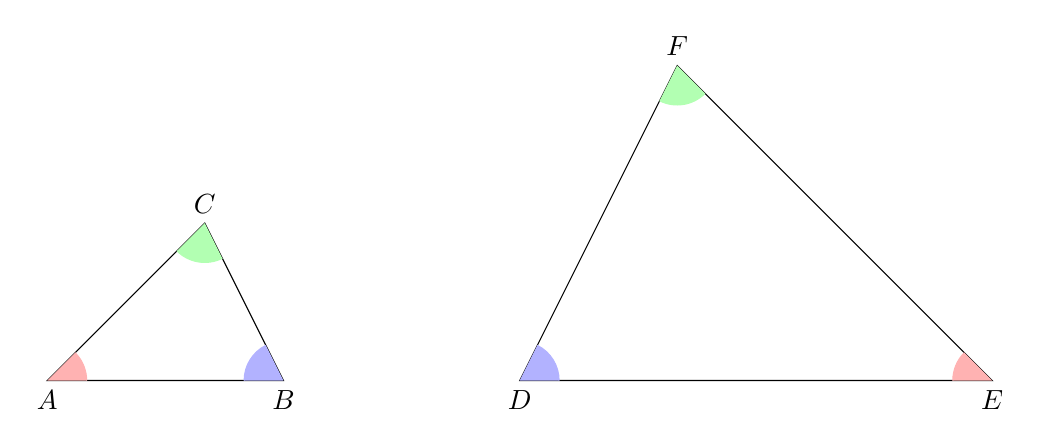
\begin{tikzpicture}
  % First triangle
  \coordinate (A) at (0,0);
  \coordinate (B) at (3,0);
  \coordinate (C) at (2,2);
  \draw (A) -- (B) -- (C) -- cycle;

  % Second triangle
  \coordinate (D) at (6,0);
  \coordinate (E) at (12,0);
  \coordinate (F) at (8,4);
  \draw (D) -- (E) -- (F) -- cycle;

  % Labeling the vertices
  \node[below] at (A) {$A$};
  \node[below] at (B) {$B$};
  \node[above] at (C) {$C$};
  \node[below] at (D) {$D$};
  \node[below] at (E) {$E$};
  \node[above] at (F) {$F$};

  \draw pic[draw=green!30,fill=green!30,angle radius=0.5cm] {angle=A--C--B};
  \draw pic[draw=green!30,fill=green!30,angle radius=0.5cm] {angle=D--F--E};
  \draw pic[draw=red!30,fill=red!30,angle radius=0.5cm] {angle=B--A--C};
  \draw pic[draw=red!30,fill=red!30,angle radius=0.5cm] {angle=F--E--D};
  \draw pic[draw=blue!30,fill=blue!30,angle radius=0.5cm] {angle=C--B--A};
  \draw pic[draw=blue!30,fill=blue!30,angle radius=0.5cm] {angle=E--D--F};
\end{tikzpicture}
\end{center}



Segitiga $ABC$ dan $DEF$ sebangun atau $ABC \sim DEF$ jika dan hanya jika minimal salah satu syarat ini terpenuhi:
\begin{enumerate}
    \item $\angle ABC = \angle DEF$ dan $\angle BAC = \angle EDF$.
    \item $\dfrac{AB}{DE} = \dfrac{BC}{EF} = \dfrac{CA}{FD}$.
    \item $\dfrac{AB}{DE} = \dfrac{BC}{EF}$ dan $\angle ABC = \angle DEF$ (sudut yang diapit dua sisi yang diperbandingkan nilainya sama)
\end{enumerate}

\subsection{Kekongruenan Segitiga}
\begin{center}
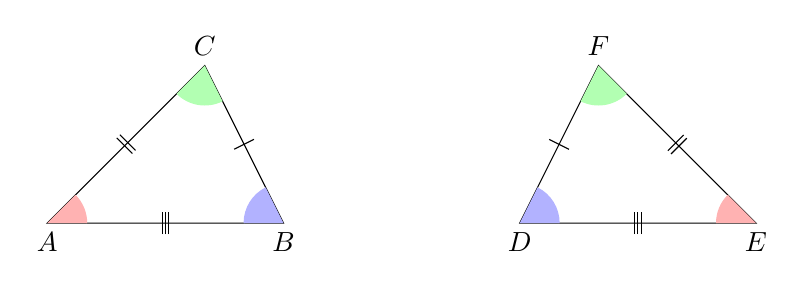
\begin{tikzpicture}
  % First triangle
  \coordinate (A) at (0,0);
  \coordinate (B) at (3,0);
  \coordinate (C) at (2,2);
  \draw (A) -- (B) -- (C) -- cycle;

  % Second triangle
  \coordinate (D) at (6,0);
  \coordinate (E) at (9,0);
  \coordinate (F) at (7,2);
  \draw (D) -- (E) -- (F) -- cycle;

  % Labeling the vertices
  \node[below] at (A) {$A$};
  \node[below] at (B) {$B$};
  \node[above] at (C) {$C$};
  \node[below] at (D) {$D$};
  \node[below] at (E) {$E$};
  \node[above] at (F) {$F$};

  \draw pic[draw=green!30,fill=green!30,angle radius=0.5cm] {angle=A--C--B};
  \draw pic[draw=green!30,fill=green!30,angle radius=0.5cm] {angle=D--F--E};
  \draw pic[draw=red!30,fill=red!30,angle radius=0.5cm] {angle=B--A--C};
  \draw pic[draw=red!30,fill=red!30,angle radius=0.5cm] {angle=F--E--D};
  \draw pic[draw=blue!30,fill=blue!30,angle radius=0.5cm] {angle=C--B--A};
  \draw pic[draw=blue!30,fill=blue!30,angle radius=0.5cm] {angle=E--D--F};

    \tkzMarkSegment[pos=.5,mark=|](C,B)
    \tkzMarkSegment[pos=.5,mark=|](D,F)
    \tkzMarkSegment[pos=.5,mark=||](C,A)
    \tkzMarkSegment[pos=.5,mark=||](E,F)
    \tkzMarkSegment[pos=.5,mark=|||](B,A)
    \tkzMarkSegment[pos=.5,mark=|||](E,D)
\end{tikzpicture}
\end{center}

Sedangkan $ABC$ dan $DEF$ dikatakan kongruen atau $\triangle ABC \cong \triangle DEF$ jika dan hanya jika $AB=DE, BC=EF, CA=FD$ atau dengan kata lain kedua segitiga tersebut sebangun dan ada salah satu sisi dari kedua segitiga tersebut yang panjangnya sama. Simpelnya kongruen = sama persis.

\subsection{Teorema Pythaogras}
Salah satu teorema paling terkenal di kalangan awam (atau setidaknya di pop culture). Diberikan segitiga $ABC$ dengan sudut $C$ siku-siku. Jika panjang sisi $AB=c$, $BC=a$, dan $CA=b$, maka berlaku
\begin{align*}
    a^2+b^2=c^2
\end{align*}
\begin{center}
    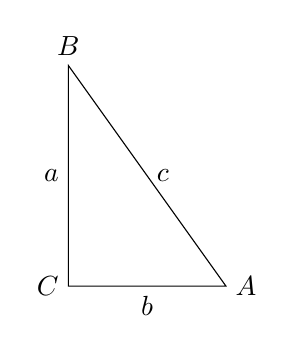
\begin{tikzpicture}
    % titik-titik segitiga
    \coordinate[label=left:$C$]  (C) at (-1.5cm,-1.cm);
    \coordinate[label=above:$B$] (B) at (-1.5cm,1.8cm);
    \coordinate[label=right:$A$] (A) at (0.5cm,-1.cm);
    
    % pembuatan segitiga
    \draw (A) -- node[right]{$c$} (B)  -- node[left]{$a$} (C) -- node[below]{$b$} cycle;
    \end{tikzpicture}
\end{center}
\input{Soal/Geometry/pythagoras}
\subsection{Trigonometri}
Banyak sih rumusnya, tapi yang paling sering dipake di olim:
\begin{enumerate}
    \item $\sin (-x) = -\sin x$.
    \item $\cos (-x) = \cos x$.
    \item $\tan(-x) = -\tan x$.
    \item $\sin^2 x + \cos^2 x = 1$.
    \item $\sin(90^\circ-x)=\sin(90^\circ+x)=\cos x$.
    \item $\sin(a \pm b) = \sin a \cos b \pm \cos a \sin b$.
    \item $\sin 2x = 2\sin x \cos x$.
    \item $\cos(a \pm b) = \cos a \cos b \mp \sin a \sin b$.
    \item $\cos 2x = \cos^2 x - \sin^2 x = 2\cos^2 x -1 = 1-2\sin^2 x$.
    \item $\tan(a \pm b) = \dfrac{\tan a \pm \tan b}{1 \mp \tan a \tan b}$.
\end{enumerate}
Cara menghafal yang gampang bisa pake "metode sumbu".

\subsection{Latihan Soal Trigonometri}
\begin{enumerate}
    \item (OSK 2022) Diberikan segitiga $ABC$ seperti di gambar, dengan panjang $AB = 2BC$ dan $BD = CD$. Jika luas segitiga $DEC$ adalah 10, luas dari segitiga $AFE$ adalah \dots

	\item Jika $A+B=45^\circ$ dan $\cos A\sin B=\frac{\sqrt{2}}{6}$, maka $\cos(B-A)=\dots$
	
	\item Nilai dari $\cos \dfrac{\pi}{7}\cdot \cos \dfrac{2\pi}{7} \cdot \cos \dfrac{4\pi}{7}$ adalah \dots
	
	\item Pada segitiga $ABC$, buktikan bahwa $\tan A + \tan B + \tan C = \tan A \tan B \tan C$.
	
	\item Tentukan nilai eksak dari $\tan 1^\circ \cdot \tan 2^\circ \cdot \tan 3^\circ \cdot \ldots \cdot \tan 89^\circ$.
	
	\item (OSK 2005) Nilai dari $\sin^8 75^\circ - \cos^8 75^\circ$ adalah \dots
\end{enumerate}


	
\end{document}